%
\subsection{Local system}
\label{sec:local-system}
In this section the local system is analyzed, considering its events, use cases,
dynamic operation and the flow of events.
%
\subsubsection{User mock-ups}
\label{sec:user-mockups}
Fig.~\ref{fig:user-mockups-local} illustrates the user mock-ups for the local
system. It intends to mimic the user interaction with the local system,
clarifying the user actions (gestures) and the respective responses, as well as
the workflow, comprising its four modes.
%
\begin{figure}[htb!]
\centering
    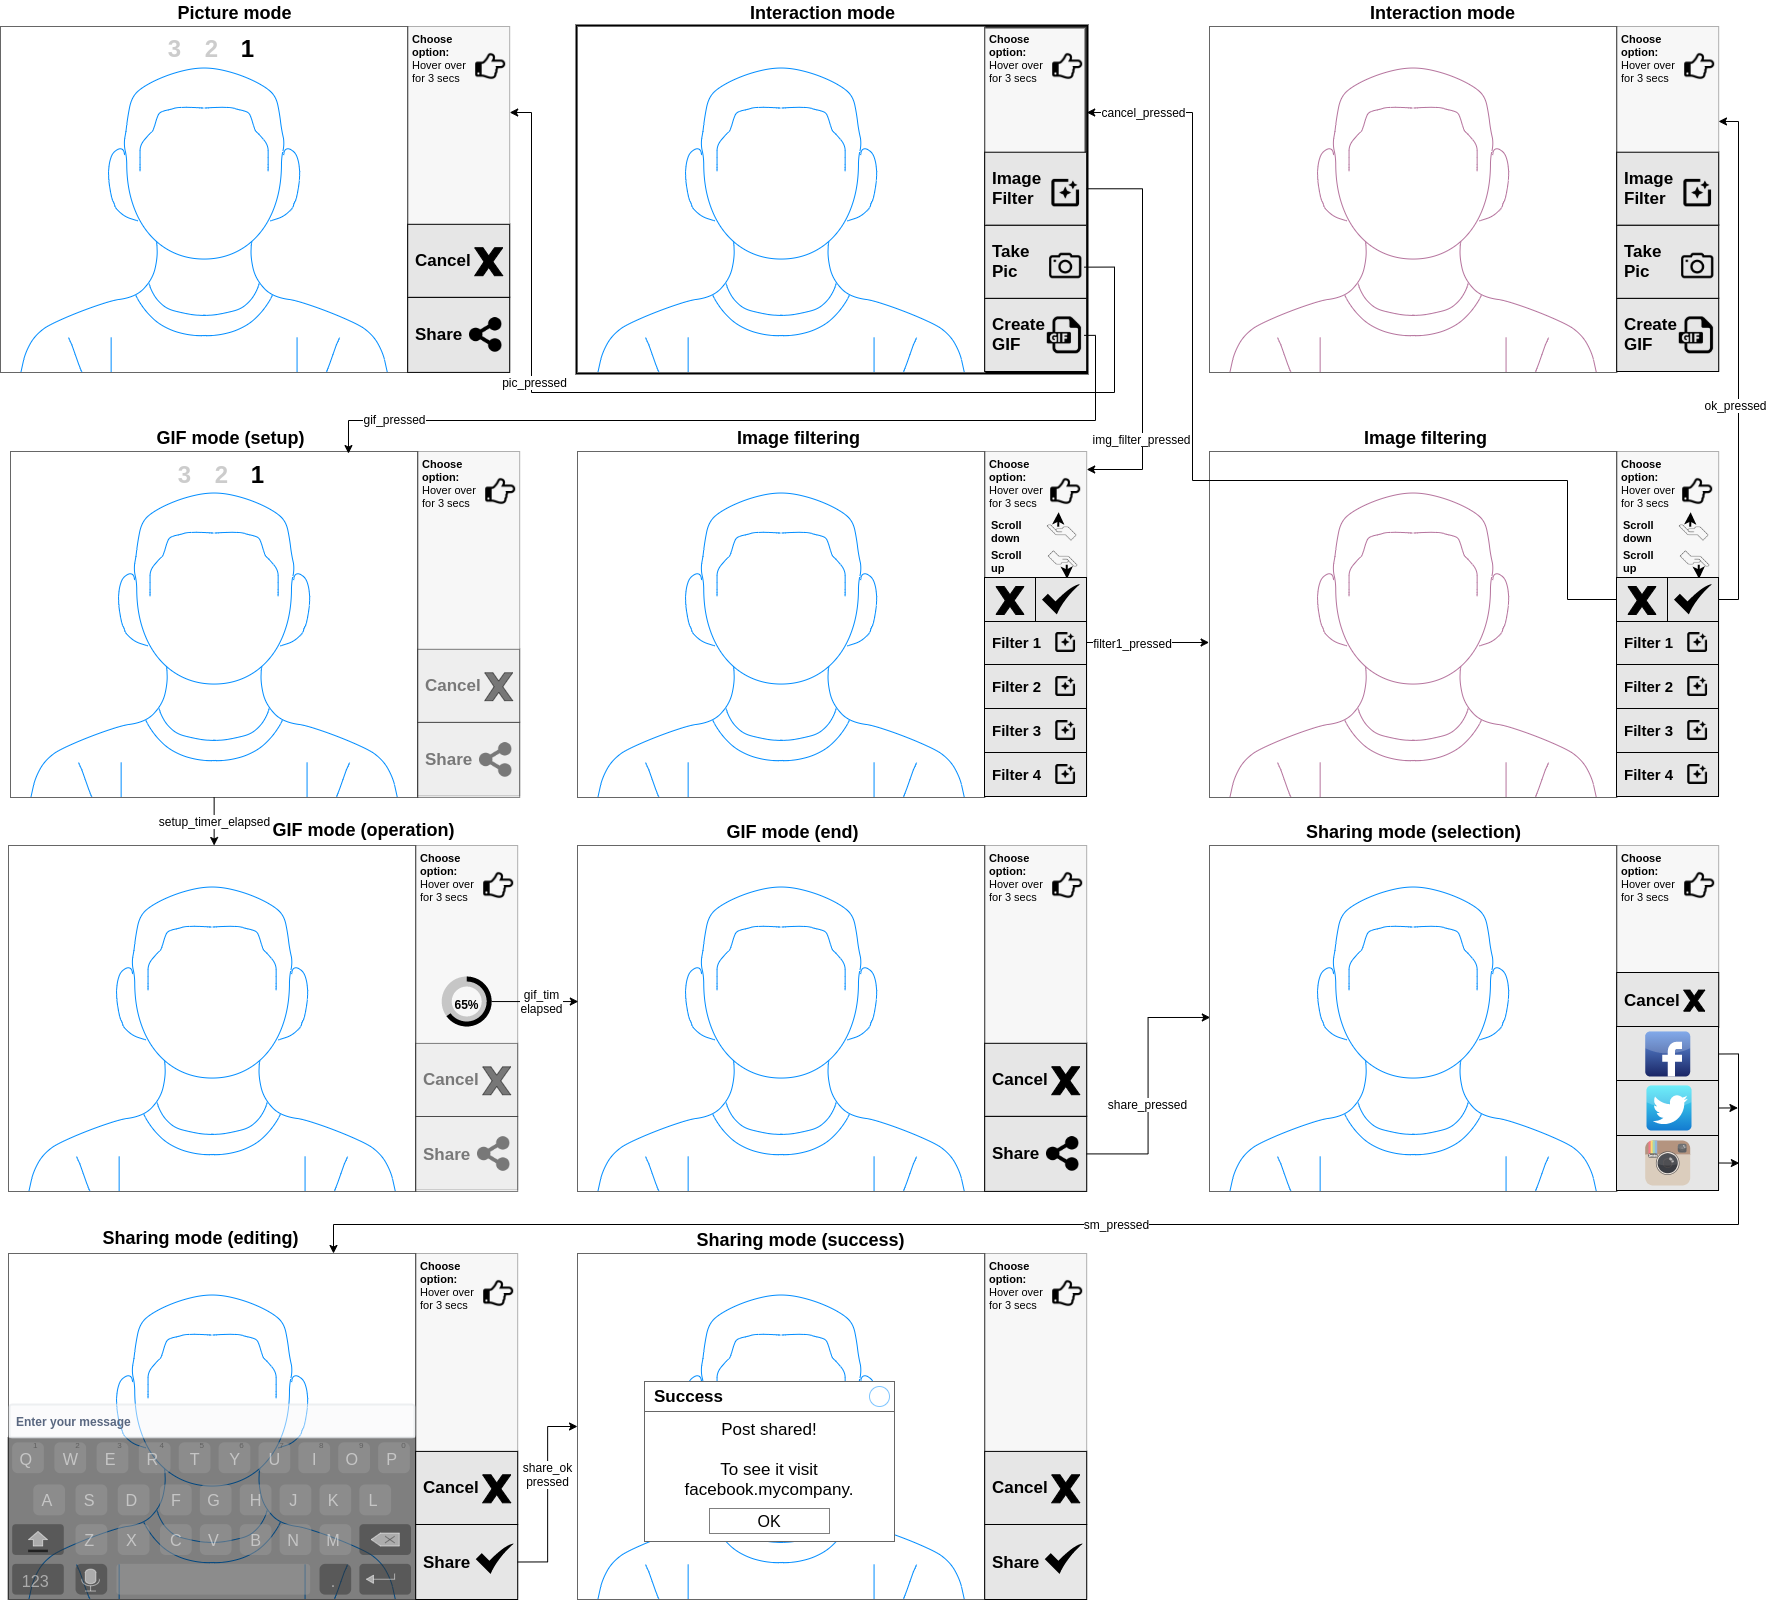
\includegraphics[width=1.0\columnwidth]{./img/user-mockups-local.png}
  \caption{User mock-ups: local system}%
\label{fig:user-mockups-local}
\end{figure}

The initial state of the \gls{mdo-l}'s~\gls{ui} is depicted in thick border
outline, after a \texttt{User} has been detected --- \texttt{Interaction
  mode}. On the left it is the camera feed and on the right the commands ribbon,
containing the hints to use the system and the available options. As it can
been, the \texttt{User} can choose an option by hovering with pointing finger
over the desired option for a designated amount of time (e.g., 3 seconds).

The workflow can be as follows:
\begin{item-c}
\item If the \texttt{User} selects the \texttt{Image filter} option, the
  \texttt{Image filtering} view is shown, presenting the options to select
  filters (which can be scrolled through palm raising/lowering), to cancel or
  accept the image filter. If a filter is selected \texttt{filter1\_pressed}, it
  is applied, and if accepted it will return to \texttt{Interaction mode},
  keeping the filter on.
\item If the \texttt{User} selects the \texttt{Take Pic} option, \texttt{Picture
  mode} is started with a timer to allow the \texttt{User} to get ready before
actually taking the picture. The \texttt{User} can \texttt{Cancel} --- returning
to main menu --- or \texttt{Share} --- starting \texttt{Sharing mode}.
\item If the \texttt{User} selects the \texttt{Create GIF} option, \texttt{GIF
    mode (setup)} is started with a timer to allow the \texttt{User} to get
  ready before actually creating the \gls{gif}. After the \texttt{setup\_timer}
  is elapsed, the \texttt{GIF mode (operation)} starts, displaying a dial with
  the \gls{gif} duration until being complete. When the \texttt{gif\_timer}
  elapses, the \gls{gif} is created, enabling the \texttt{User} to
  \texttt{Cancel} --- returning to main menu --- or to \texttt{Share} ---
  starting \texttt{Sharing mode}.
\item Lastly, in the \texttt{Sharing mode}, the \texttt{User} can
  \texttt{Cancel} --- returning to main menu --- or select the
  social media network. After selecting the social media, the \texttt{User} can
  edit the post by entering its customized message and, if \texttt{Share} is
  pressed, a message box will appear displaying the status of the post sharing
  --- \texttt{Success} or \texttt{Error}.
\end{item-c}
%
\subsubsection{Events}%
\label{sec:events}
Table~\ref{tab:events-local} presents the most relevant events for the
\texttt{Local system}, categorizing them by their source and synchrony and
linking it to the system's intended response. A further division is done
separating \emph{\gls{ui} events} from the remaining ones.

\begingroup
\renewcommand{\arraystretch}{0.7} % Default value: 1
\begin{table}[hbt!]
% Please add the following required packages to your document preamble:
% \usepackage{booktabs}
\centering
\caption{Events: local system}
\label{tab:events-local}
\begin{tabular}{@{}llll@{}}
\toprule
\textbf{Event}            & \textbf{System response}                                                                              & \textbf{Source}   & \textbf{Type} \\ \midrule
Power on                  & \begin{tabular}[c]{@{}l@{}}Initialize sensors and go \\ to Normal mode\end{tabular}                   & System maintainer & Asynchronous  \\ \midrule
User detected             & \begin{tabular}[c]{@{}l@{}}Turn on camera feed and \\ go to Interaction mode\end{tabular}             & User              & Asynchronous  \\ \midrule
Command received          & Parse it and respond                                                                                  & Remote Server     & Asynchronous  \\ \midrule
Database update           & \begin{tabular}[c]{@{}l@{}}Request update of internal \\ databases to Remote Server\end{tabular}      & Database manager  & Asynchronous  \\ \midrule
Enable fragrance diffuser & \begin{tabular}[c]{@{}l@{}}Enable fragrance diffusion for \\ a predefined period of time\end{tabular} & Local System      & Synchronous   \\ \midrule
Video ended               & \begin{tabular}[c]{@{}l@{}}Playback the next video \\ on the queue\end{tabular}                       & Local System      & Synchronous   \\ \midrule
Check WiFi connection     & Periodically check WiFi connection                                                                    & Local System      & Synchronous   \\ \midrule
\multicolumn{4}{c}{\textbf{UI events}}                                                                                                                                \\ \midrule
Option selected           & \begin{tabular}[c]{@{}l@{}}Track the option selected and \\ inform the UI engine\end{tabular}         & User              & Asynchronous  \\ \midrule
Image filter pressed      & Go to Image filter view                                                                               & User              & Asynchronous  \\ \midrule
Filter selected           & Detect User's face and apply filter                                                                   & User              & Asynchronous  \\ \midrule
Pic pressed               & Go to Picture mode                                                                                    & User              & Asynchronous  \\ \midrule
Pic setup elapsed         & Take picture                                                                                          & Local System      & Synchronous   \\ \midrule
GIF pressed               & Go to GIF mode                                                                                        & User              & Asynchronous  \\ \midrule
GIF setup elapsed         & Go to GIF operation                                                                                   & Local System      & Synchronous   \\ \midrule
GIF operation elapsed     & Finish GIF                                                                                            & Local System      & Synchronous   \\ \midrule
Share mode pressed        & Go to Sharing mode (selection)                                                                        & User              & Asynchronous  \\ \midrule
Keyboard pressed          & Give feedback to user                                                                                 & User              & Asynchronous  \\ \midrule
Share post pressed        & Upload post to designated social media                                                                & User              & Asynchronous  \\ \midrule
Share post status         & Inform user about shared post status                                                                  & Cloud             & Asynchronous  \\ \bottomrule
\end{tabular}
\end{table}
\endgroup
%
\subsubsection{Use cases}
\label{sec:use-cases}
Fig.~\ref{fig:use-cases-local} depicts the use cases diagram for the
\texttt{Local System}, describing how the system should respond under various
conditions to a request from one of the stakeholders to deliver a specific
goal.

The \texttt{Admin} interacts with the \texttt{Remote Client} (through its
\gls{ui}) requesting the \texttt{Remote Server} to process commands, getting the
state of the device, adding a video or selecting the fragrance. Additionally,
the \texttt{Admin} may test the operation of the device: play video, test audio,
nebulize fragrance or test the camera. This last one tests the main
functionalities the \texttt{User} also utilizes, namely: select image filter,
apply/reject image filter, take picture, create \gls{gif} or share multimedia on
the social media.

A precondition for the interaction of the \texttt{Admin} with the \texttt{Local System} is the establishment of a remote
connection between the \texttt{Remote Server} and the \texttt{Local system},
verifying its credentials. However, there is another important use case for this
remote connection: the update of the \texttt{Local System}'s internal databases
from the \texttt{Remote server} which will sent appropriate commands for this purpose.
%
\begin{figure}[htb!]
\centering
    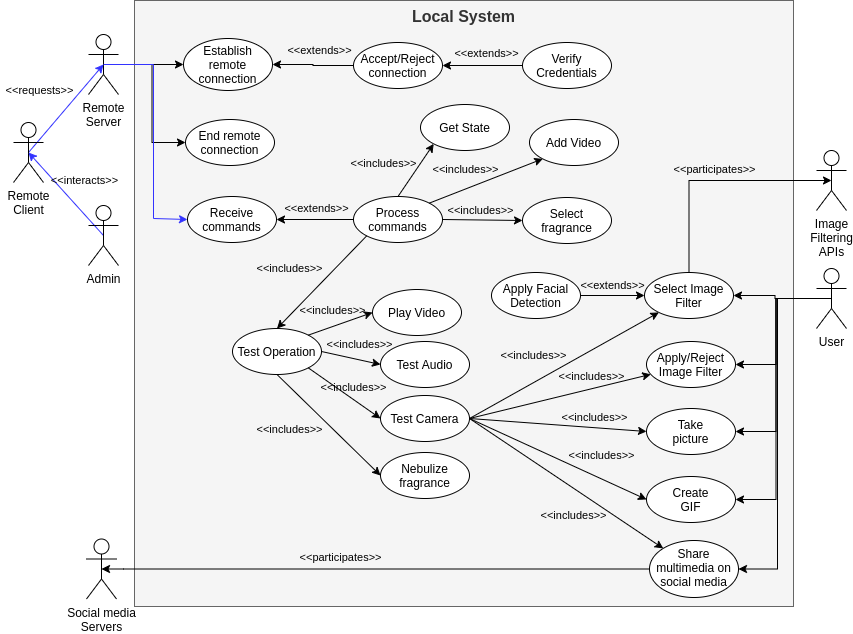
\includegraphics[width=0.85\columnwidth]{./img/use-cases-local.png}
  \caption{Use cases diagram: local system}%
\label{fig:use-cases-local}
\end{figure}
%
\subsubsection{Dynamic operation}
\label{sec:dyn-oper}
Fig.~\ref{fig:state-mach-local} depicts the state machine diagram for the
\texttt{Local System}, illustrating its dynamic behavior.
%
\begin{figure}[htb!]
\centering
    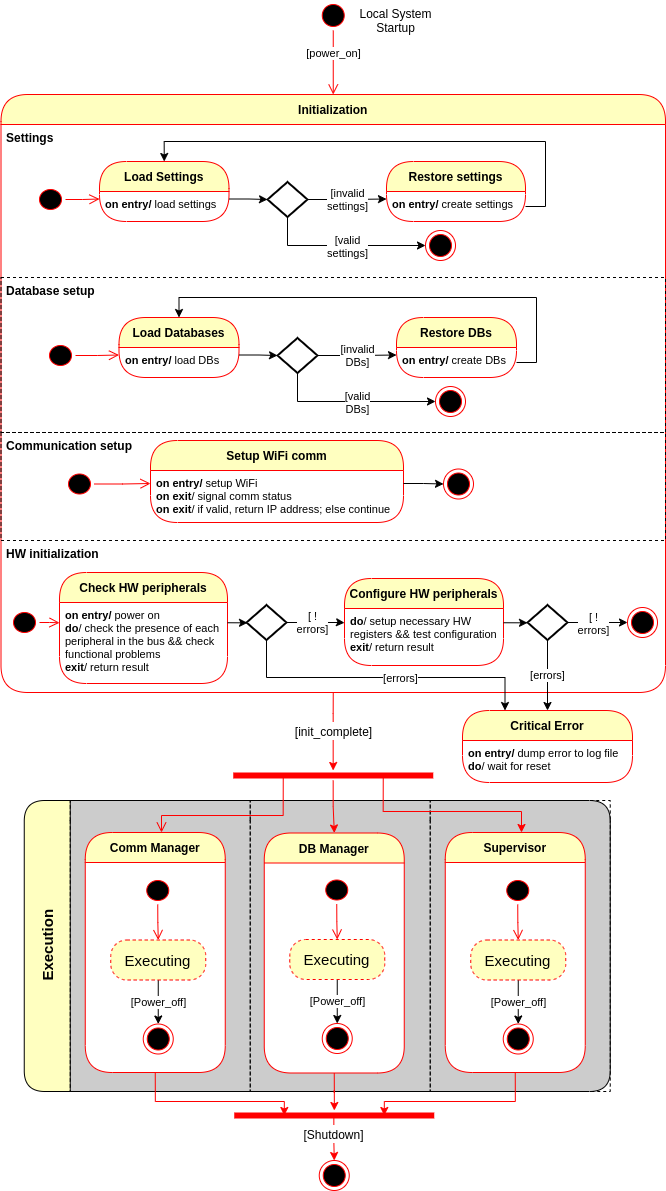
\includegraphics[width=0.7\columnwidth]{./img/state-mach-local.png}
  \caption{State machine diagram: local system}%
\label{fig:state-mach-local}
\end{figure}
%

There are two main states:
\begin{item-c}
\item \emph{\texttt{Initialization}}: the device is initialized. The settings
  and \gls{db}s are loaded and if invalid they are restored. The WiFi
  communication is setup, signaling the communication status and if valid, an
  \gls{ip} address is returned. Lastly, the \gls{hw} is initialized, checking
  its presence, configuring it and testing the configuration: if any error
  occurs the device goes into the \texttt{Critical Error} state, dumping the
  error to a log file and waiting for reset; otherwise, the initialization is
  complete.
\item \emph{\texttt{Execution}}: after the initialization is successful, the
  system goes into the \texttt{Execution} macro composite state with several
  concurrent activities, modeled as composite states too. However, it should be
  noted that there is only one actual state for the device, although at the
  perceivable time scale they appear to happen simultaneously. These activities
  are communication management (\texttt{Comm Manager}), \gls{db} management
  (\texttt{DB manager}), and application supervision (\texttt{Supervisor}), and
  are executed forever until system's power off. They are detailed next.
\end{item-c}
%
\paragraph{\emph{Communication Manager}}
Fig.~\ref{fig:state-mach-local-comm} depicts the state machine diagram for the
\texttt{Comm Manager} component. Upon successful initialization the
\texttt{Comm Manager} goes to \texttt{Idle}, listening for incoming
connections. When a remote node tries to connects, it makes a connection request
which can be accepted or denied. If the connection is accepted and the node
authenticates successfully the \texttt{Comm Manager} is ready for bidirectional
communication. When a message is received from the remote node, it is written to
\texttt{TX msg queue} and the \texttt{Supervisor} is notified. When a message
must be sent to the remote, it is read from the \texttt{TX msg queue} and sent
to the recipient. If the connection goes down, it is restarted, going into
\texttt{Idle} state again.
%
\begin{figure}[htb!]
\centering
    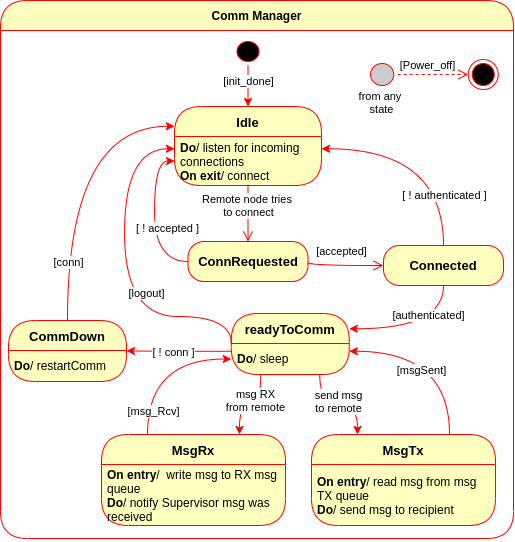
\includegraphics[width=0.6\columnwidth]{./img/state-mach-local-comm.png}
  \caption{State machine diagram: local system --- Comm Manager}%
\label{fig:state-mach-local-comm}
\end{figure}
%
%
\paragraph{\emph{Database Manager}}
Fig.~\ref{fig:state-mach-local-db} depicts the state machine diagram for the
\texttt{DB Manager} component. Upon successful initialization the
\texttt{DB Manager} goes to \texttt{Idle}, waiting for incoming \gls{db}
requests.
When a request arrives, it is parsed, checking its validity. If the request is a
\gls{db} query, a transaction is read from the respective \gls{db} to the
\texttt{RX transaction queue} and the \texttt{Supervisor} is notified that there
is a transaction to read. Otherwise, if the request is a \gls{db} update
the transaction is written from the \texttt{TX transaction queue} to the
\gls{db} and the \texttt{Supervisor} is notified that the \gls{db} was updated.
%
\begin{figure}[htb!]
\centering
    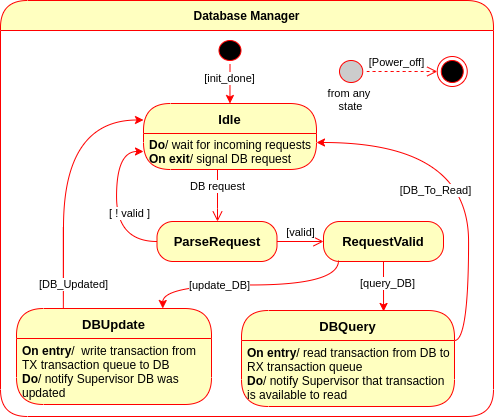
\includegraphics[width=0.6\columnwidth]{./img/state-mach-local-db.png}
  \caption{State machine diagram: local system --- \gls{db} Manager}%
\label{fig:state-mach-local-db}
\end{figure}
%
%
\paragraph{\emph{Supervisor}}
Fig.~\ref{fig:state-mach-local-superv} depicts the state machine diagram for the
\texttt{Supervisor} component, comprising two tasks running in
`parallel' (Fig.~\ref{fig:state-mach-local-superv-main}):
\begin{item-c}
%
\item \emph{\texttt{Request Handler}} (Fig.~\ref{fig:state-mach-local-superv-req}): handles incoming requests from the
  \texttt{Remote server}. When a request arrives, it is parsed, and, if valid,
  the appropriate callback is triggered, processing the request and returning
  its output.
%  
\item \emph{\texttt{Mode manager}} (Fig.~\ref{fig:state-mach-local-superv-mode}): Upon successful initialization the
  \texttt{Mode Manager} goes to \texttt{Idle}, and it is `awake' if it is time
  to play the advertisements or if a user is detected. If the former is
  verified--- \texttt{Normal mode} --- the device retrieves video
  and fragrance data from the \gls{db} and plays video and nebulizes
  fragrance. If the latter is verified --- \texttt{Interaction mode} the device
  turns on the camera and mirrors the feed on the display, waiting for a
  recognizable gesture.

  If the \texttt{User} choose to select an image filter,
  take a picture or create a \gls{gif}, the device goes into \texttt{Multimedia
    mode}, returning back to \texttt{Interaction mode} after its exit condition
  or after a timeout.

  Lastly, if the \texttt{User} chooses to share the image or
  \gls{gif} created, it must select the social media network, edit the post to
  enter some message and confirm the sharing, returning to \texttt{Interaction
    mode}. If no user interaction happens for a while, the device returns back
  to \texttt{Idle} mode.
%
\end{item-c}
%
%\begin{figure}[htb!]
%\centering
%    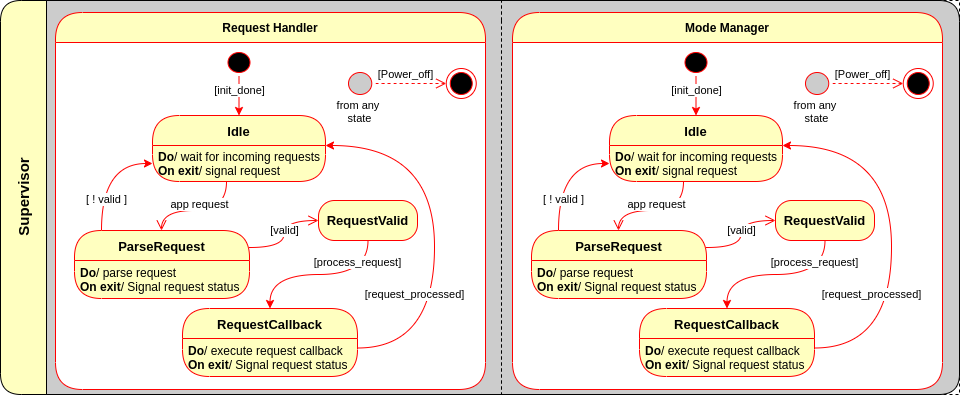
\includegraphics[width=1.0\columnwidth]{./img/state-mach-local-superv.png}
%  \caption{State machine diagram: local system --- Supervisor}%
%\label{fig:state-mach-local-superv}
%\end{figure}
%
\begin{figure}[htb!]
  \centering
  % 
  \begin{subfigure}[t]{.4\textwidth}
  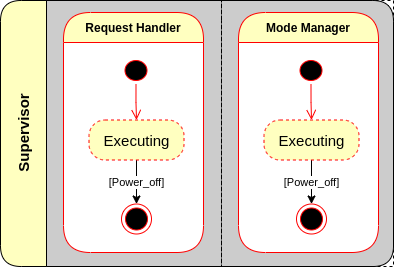
\includegraphics[width=\textwidth]{img/state-mach-local-superv-main.png}%
  \caption{main}%
  \label{fig:state-mach-local-superv-main}
\end{subfigure}
%
\hspace{.05\textwidth}
%
  \begin{subfigure}[t]{.42\textwidth}
  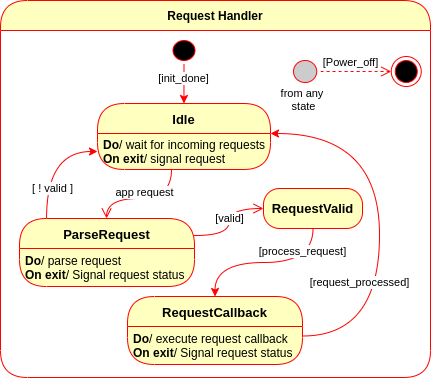
\includegraphics[width=\textwidth]{img/state-mach-local-superv-req.png}%
  \caption{Request Handler}%
  \label{fig:state-mach-local-superv-req}
\end{subfigure}
  %
%
%\vspace{.1\textwidth}
%
  \begin{subfigure}{.9\textwidth}
  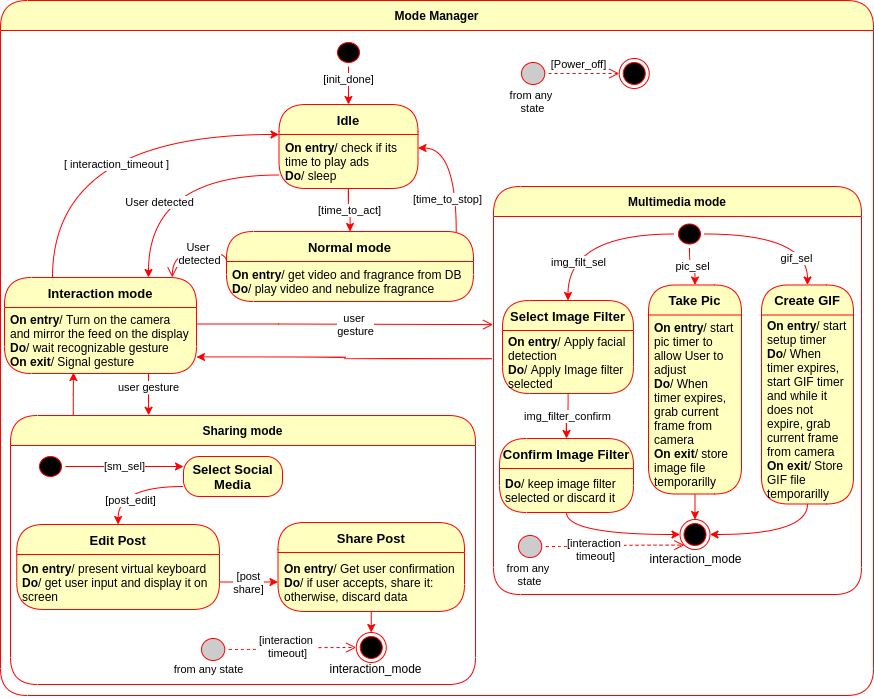
\includegraphics[width=\textwidth]{img/state-mach-local-superv-mode.png}%
  \caption{Mode Manager}%
  \label{fig:state-mach-local-superv-mode}
\end{subfigure}
  % 
  \caption{State machine diagram: local system --- Supervisor}%
  \label{fig:state-mach-local-superv}
\end{figure}
%
%
\subsubsection{Flow of events}%
\label{sec:flow-events}
The flow of events throughout the system is described using a sequence diagram,
comprising the interactions between the most relevant system's entities. It is
usually pictured as the visual representation of an use case. The main sequence
diagrams are illustrated next.

\paragraph{\emph{Normal mode}}
Fig.~\ref{fig:seq-local-normal-mode} depicts the \texttt{Normal
  mode}'s sequence diagram. The blue area delimits the \texttt{\gls{mdo-l}}
system, comprising the \texttt{Local System Back-End}.
%
\begin{figure}[htb!]
  \centering
  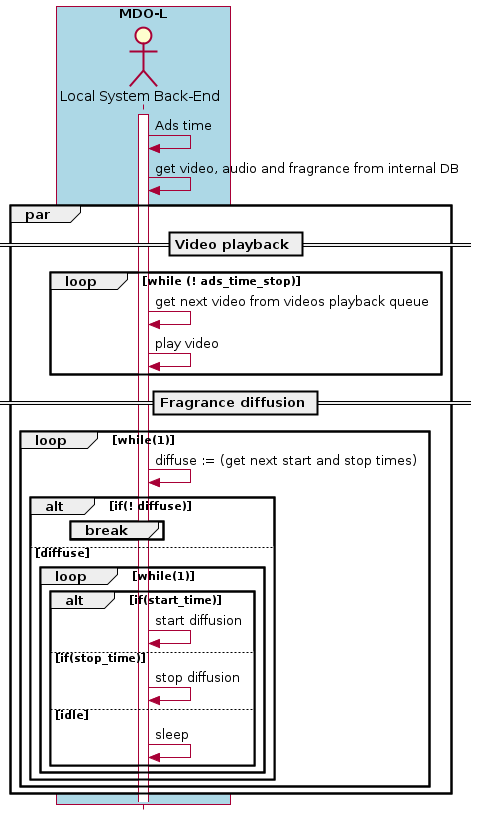
\includegraphics[width=0.5\columnwidth]{./img/seq-local-normal-mode.png}
  \caption{Sequence diagram: local system --- Normal mode}%
\label{fig:seq-local-normal-mode}
\end{figure}

When its time to play the advertisements, the \texttt{Normal} mode is activated,
retrieving video, audio and fragrance from the internal \gls{db}. Then two
parallel activities are executed:
\begin{item-c}
\item \emph{Video playback}: while its time to play the advertisements, a video
  is played from the video list. When it finishes, it moves the next video in
  the playback queue.
\item \emph{Fragrance diffusion}: while there are timestamps for fragrance
  diffusion, diffuse fragrance between start and stop times and sleep on the
  other occasions.
\end{item-c}
%
\paragraph{\emph{Interaction mode}}
Fig.~\ref{fig:seq-local-interaction-mode} depicts the \texttt{Interaction
  mode}'s sequence diagram. The blue area delimits the \texttt{\gls{mdo-l}}
system, comprising the \texttt{Gesture Recognition Engine}, the \texttt{UI
  engine} and the \texttt{Local System Back-End}.
%
\begin{figure}[htb!]
  \centering
  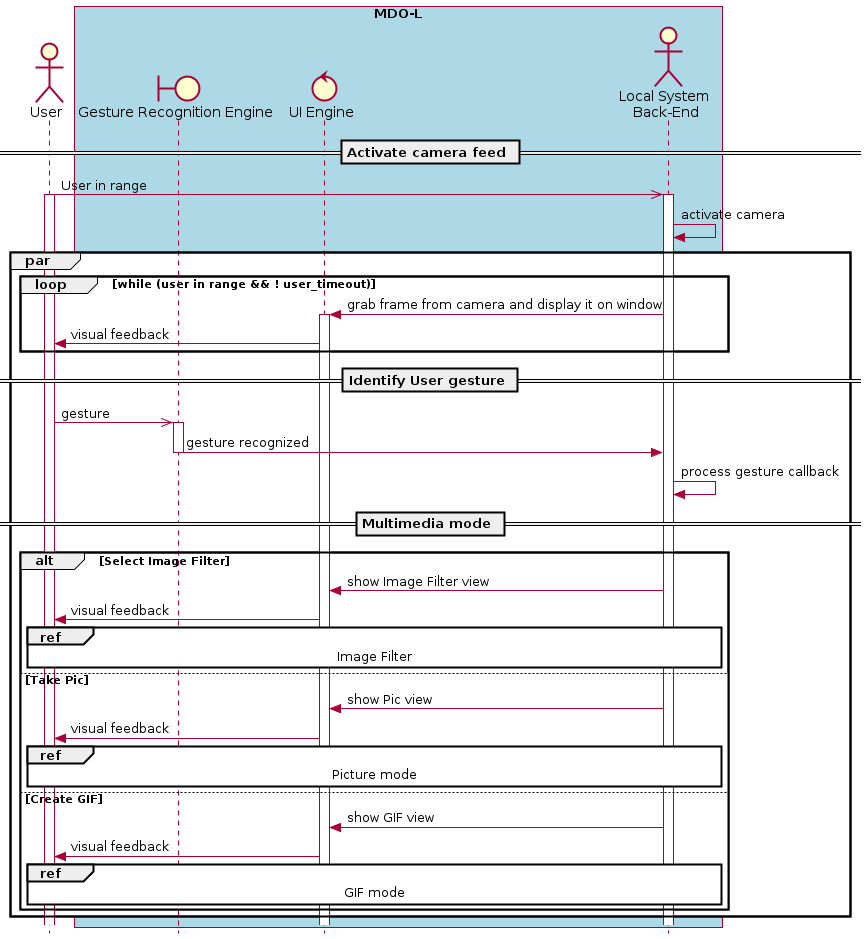
\includegraphics[width=0.8\columnwidth]{./img/seq-local-interaction-mode.png}
  \caption{Sequence diagram: local system --- Interaction mode}%
\label{fig:seq-local-interaction-mode}
\end{figure}

When the \texttt{User} is in range (asynchronous event), the camera is
activated, and two parallel activities are executed:
\begin{item-c}
\item \emph{mirror camera feed}: while the \texttt{User} is in range and
active, the \texttt{UI engine} will grab frame from the camera and display it on
the window providing visual feedback to the \texttt{User}.
\item \emph{gesture recognition and processing}: if a gesture is recognized by
  the \texttt{Gesture Recognition Engine} it is dispatched to the \texttt{Local
    System Back-End} which will process it according to the following cases:
  \texttt{Select Image filter}, \texttt{Take Pic}, and \texttt{Create GIF},
  showing the respective view in the \gls{ui} and triggering the associate
  sequence diagram (indicated by the \texttt{ref} keyword).
\end{item-c}
%
\paragraph{\emph{Multimedia mode}}
Fig.~\ref{fig:seq-local-multimedia-mode-sel-filt} through
Fig.~\ref{fig:seq-local-multimedia-mode-create-gif} depicts the
\texttt{Multimedia mode}'s sequence diagrams, namely:
\begin{item-c}
\item \emph{\texttt{Select image filter}} (Fig.~\ref{fig:seq-local-multimedia-mode-sel-filt}): after the \texttt{Image
  filter view} is presented to the \texttt{User}, he/she can make a gesture to
select the filter, which upon being recognized by the \texttt{Gesture
  Recognition Engine} it is dispatched by the \texttt{UI Engine} to the
\texttt{Local System back-end}. Facial recognition is then applied, and while
the filter is active, a request is made to \texttt{Image Filtering APIs} to
apply the designated filter, showing it to the \texttt{User} --- \texttt{Apply
  filter} reference.

If the \texttt{User} accepts the filter, it returns to \texttt{Interaction mode}
with the filter simultaneously on (\texttt{Apply filter}). Otherwise, it the
\texttt{User} cancels it, it simply returns to \texttt{Interaction mode}.
% 
\item \emph{\texttt{Take picture}}: after \texttt{Picture mode} is initiated,
  the \texttt{Local System back-end} starts a timer to allow the \texttt{User}
  to get in position, and while the timer is running, the time remaining is
  presented to the \texttt{User}. When the timer elapses the picture is stored
  internally.
%
\item \emph{\texttt{Create GIF}}: after \texttt{\gls{gif} mode} is initiated,
  the \texttt{Local System back-end} starts a timer to allow the \texttt{User}
  to get in position, and while the timer (\texttt{gif\_setup\_timer}) is running, the time remaining is
  presented to the \texttt{User}. When the timer elapses the \gls{gif} creation
  can start, with another timer (\texttt{gif\_oper\_timer}) being started, and while the timer is running
  the remaining time is shown to \texttt{User} but in a dial form. When this
  timer elapses the \gls{gif} is stored internally.
\end{item-c}
%
\begin{figure}[htb!]
  \centering
  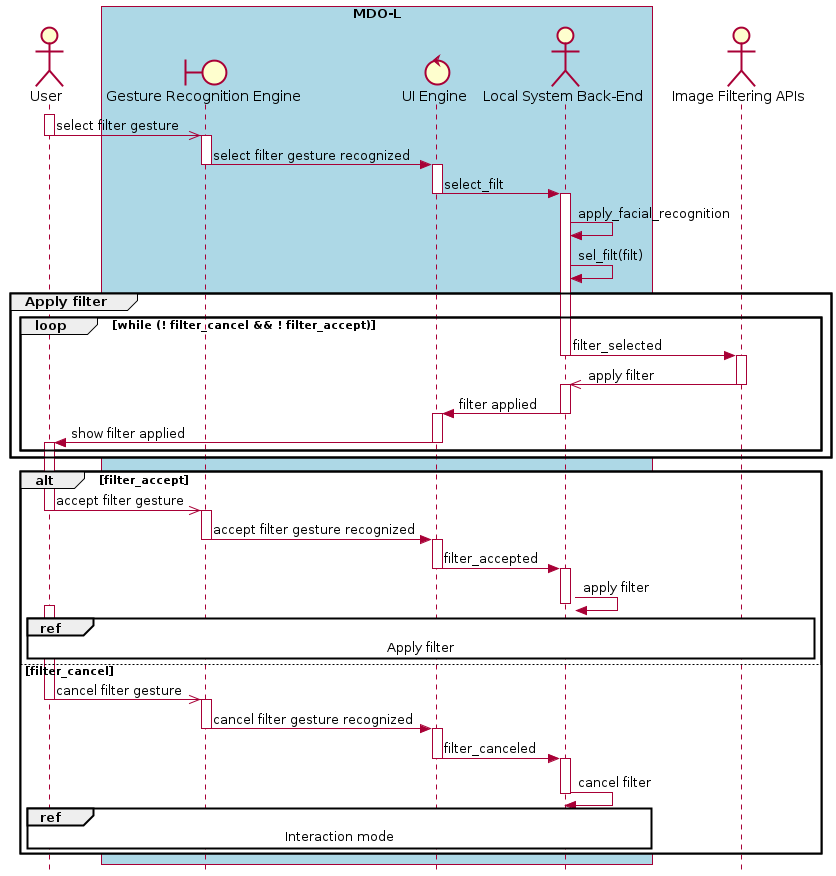
\includegraphics[width=0.8\columnwidth]{./img/seq-local-multimedia-mode-sel-filt.png}
  \caption{Sequence diagram: local system --- Multimedia mode (select image filter)}%
\label{fig:seq-local-multimedia-mode-sel-filt}
\end{figure}
%
\begin{figure}[htb!]
  \centering
  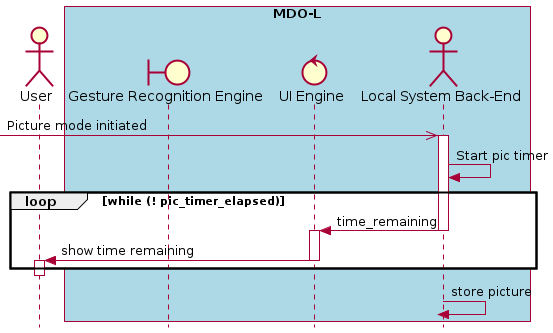
\includegraphics[width=0.55\columnwidth]{./img/seq-local-multimedia-mode-take-pic.png}
  \caption{Sequence diagram: local system --- Multimedia mode (take picture)}%
\label{fig:seq-local-multimedia-mode-take-pic}
\end{figure}
%
\begin{figure}[htb!]
  \centering
  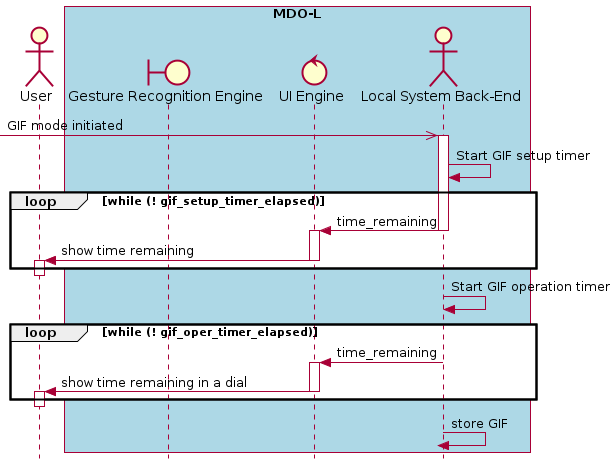
\includegraphics[width=0.55\columnwidth]{./img/seq-local-multimedia-mode-create-gif.png}
  \caption{Sequence diagram: local system --- Multimedia mode (create \gls{gif})}%
\label{fig:seq-local-multimedia-mode-create-gif}
\end{figure}
%
\paragraph{\emph{Sharing mode}}
Fig.~\ref{fig:seq-local-sharing-mode} depicts the \texttt{Sharing
  mode}'s sequence diagram.
%The blue area delimits the \texttt{\gls{mdo-l}}
%system, comprising the \texttt{Gesture Recognition Engine}, the \texttt{UI
%  engine} and the \texttt{Local System Back-End}.
%
\begin{figure}[htb!]
  \centering
  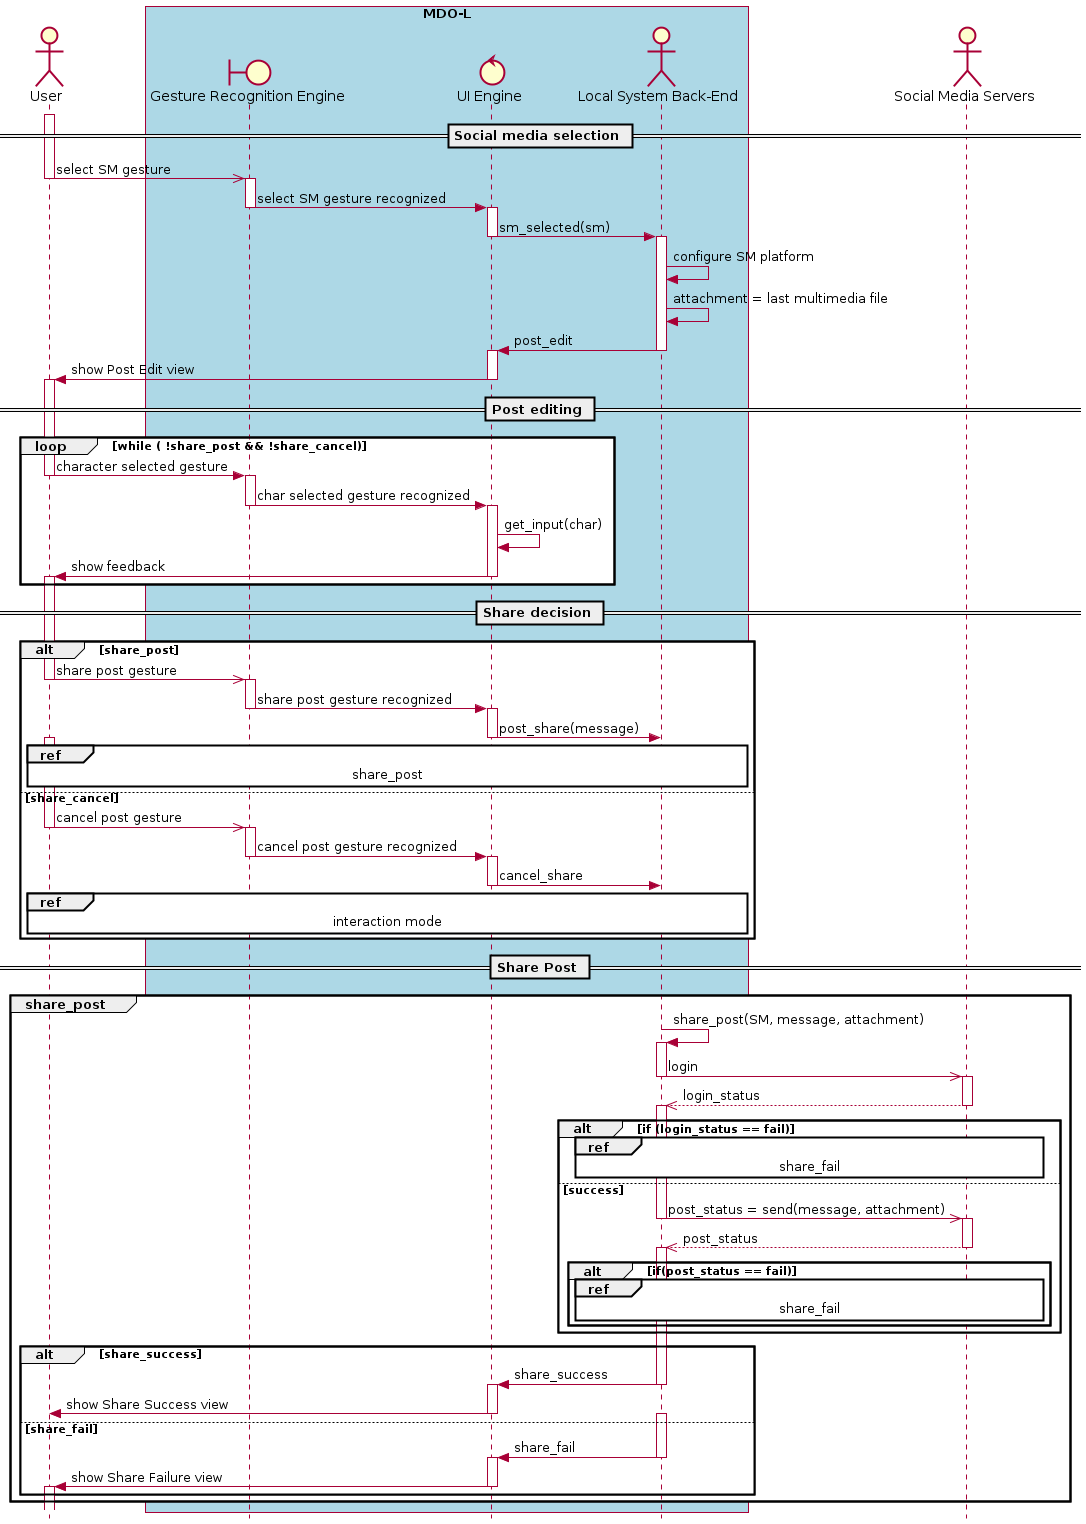
\includegraphics[width=0.9\columnwidth]{./img/seq-local-sharing-mode.png}
  \caption{Sequence diagram: local system --- Sharing mode}%
\label{fig:seq-local-sharing-mode}
\end{figure}

The \texttt{User} starts by selecting the social media platform (with a
gesture), which upon being recognized is dispatched to the \texttt{Local System
  back-end} identifying the social media selected. Then, the social media
parameters are configured and the \texttt{attachment} is set to the last
multimedia file. After social media configuration, the \texttt{Post Edit} view
is shown to the \texttt{User}.

In the \texttt{Post editing} mode, while the \texttt{User} does not decide to
share or cancel the post, the selected character from the virtual keyboard is
visually feed back to the \texttt{User}.

When the \texttt{User} decides to share or cancel the post, it will trigger
\texttt{share\_post} or \texttt{cancel\_post} callbacks, with the latter going
into \texttt{Interaction mode}.

Upon triggering the \texttt{share\_post} callback, \texttt{Local System
  back-end} tries to perform the login in the required social media platform,
requesting it to one of its servers. If the login succeeds, the post is sent to
\texttt{Social Media servers}, which will return its status. Upon completion a
dialog box will be presented to the \texttt{User}, informing it of share post
status: success or failure (in case the login or the post transmission fails).
%
%%% Local Variables:
%%% mode: latex
%%% TeX-master: "../../../dissertation"
%%% End: